\documentclass{article}
% Shared style for the LUMEN manuscript diagrams (\input by every fig_*.tex; class: article).
% Uses only fonts and packages of a basic TeX installation (Computer Modern Sans), so compiling
% never triggers a package download. Each figure is wrapped in the lumenfig environment, which
% ships the picture out as a single page cropped to the drawing plus a 3 pt margin.
\usepackage{amsmath,amssymb}
\renewcommand{\familydefault}{\sfdefault}
\usepackage{tikz}
\usetikzlibrary{positioning,arrows.meta,fit,backgrounds,calc,shapes.geometric,decorations.pathreplacing}
\pagestyle{empty}

\newsavebox{\lumenfigbox}
\newenvironment{lumenfig}%
  {\begin{lrbox}{\lumenfigbox}}%
  {\end{lrbox}%
   \pdfpagewidth=\dimexpr\wd\lumenfigbox+6pt\relax
   \pdfpageheight=\dimexpr\ht\lumenfigbox+\dp\lumenfigbox+6pt\relax
   \hoffset=-1in\voffset=-1in
   \shipout\vbox{\kern3pt\hbox{\kern3pt\usebox{\lumenfigbox}}}}

% palette: physics (blue), learning (green), data (amber), reporting (violet), neutral ink
\definecolor{ink}{HTML}{1F2933}
\definecolor{muted}{HTML}{52606D}
\definecolor{rule}{HTML}{CBD2D9}
\definecolor{phyE}{HTML}{3B6EA8}\definecolor{phyF}{HTML}{E8F1FB}
\definecolor{lrnE}{HTML}{3C8C5A}\definecolor{lrnF}{HTML}{EAF6EE}
\definecolor{datE}{HTML}{B7791F}\definecolor{datF}{HTML}{FDF3E4}
\definecolor{outE}{HTML}{6B4FA0}\definecolor{outF}{HTML}{F3EEFB}
\definecolor{grey}{HTML}{9AA5B1}

\tikzset{
  >={Stealth[length=2.4mm,width=1.8mm]},
  every node/.style={font=\footnotesize, text=ink},
  box/.style={draw, rounded corners=2.5pt, line width=0.7pt, align=center, inner sep=4pt,
    execute at begin node={\hyphenpenalty=10000\exhyphenpenalty=10000}},
  phy/.style={box, draw=phyE, fill=phyF},
  lrn/.style={box, draw=lrnE, fill=lrnF},
  dat/.style={box, draw=datE, fill=datF},
  rep/.style={box, draw=outE, fill=outF},
  neutral/.style={box, draw=grey, fill=white},
  flow/.style={->, line width=0.8pt, draw=ink},
  soft/.style={->, line width=0.7pt, draw=muted, dashed},
  title/.style={font=\footnotesize\bfseries},
  note/.style={font=\scriptsize, text=muted, align=center},
  stage/.style={draw=rule, rounded corners=4pt, line width=0.6pt, dashed, inner sep=6pt},
  stagelabel/.style={font=\scriptsize\bfseries, text=muted, anchor=south west, inner sep=1pt},
}

% feature map drawn as a slab: width ~ channels, height ~ band length
\newcommand{\fmap}[6]{% name, x (cm), width (mm), height (mm), fill, shape label
  \node[draw=#5!70!black, fill=#5, line width=0.5pt, minimum width=#3mm, minimum height=#4mm, inner sep=0pt] (#1) at (#2,0) {};
  \node[font=\scriptsize, text=ink] at (#1 |- 0,-1.95) {#6};}
\begin{document}
\begin{lumenfig}
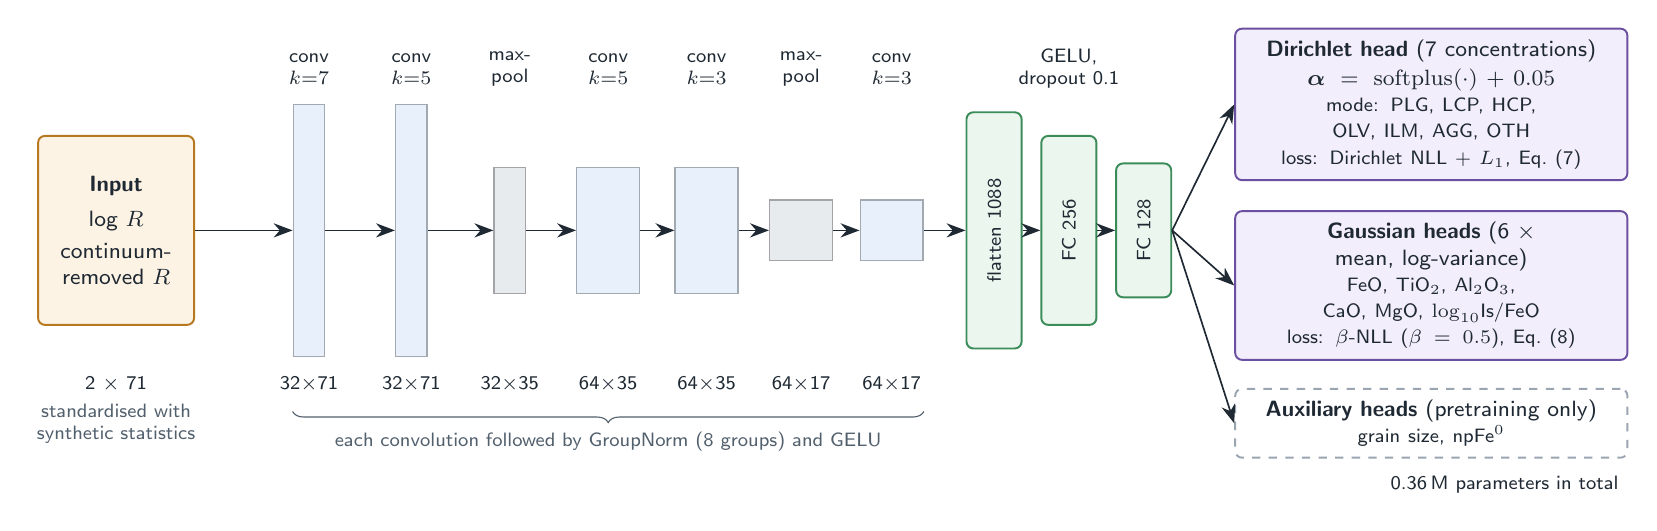
\begin{tikzpicture}
\colorlet{cvC}{phyF}\colorlet{plC}{rule!45}

% ---- input
\node[dat, text width=17mm, minimum height=24mm] (in) at (0,0) {\textbf{Input}\\[3pt]log $R$\\[2pt]continuum-\\removed $R$};
\node[font=\scriptsize, text=ink] at (in |- 0,-1.95) {2 $\times$ 71};
\node[note] at (in |- 0,-2.45) {standardised with\\synthetic statistics};

% ---- convolutional body (widths ~ channels, heights ~ bands)
\fmap{c1}{2.45}{4}{32}{cvC}{32$\times$71}
\fmap{c2}{3.75}{4}{32}{cvC}{32$\times$71}
\fmap{p1}{5.00}{4}{16}{plC}{32$\times$35}
\fmap{c3}{6.25}{8}{16}{cvC}{64$\times$35}
\fmap{c4}{7.50}{8}{16}{cvC}{64$\times$35}
\fmap{p2}{8.70}{8}{7.7}{plC}{64$\times$17}
\fmap{c5}{9.85}{8}{7.7}{cvC}{64$\times$17}
\foreach \a/\b in {in/c1,c1/c2,c2/p1,p1/c3,c3/c4,c4/p2,p2/c5} \draw[flow, line width=0.6pt] (\a.east) -- (\b.west);

\foreach \n/\t in {c1/{conv\\$k{=}7$},c2/{conv\\$k{=}5$},p1/{max-\\pool},c3/{conv\\$k{=}5$},c4/{conv\\$k{=}3$},p2/{max-\\pool},c5/{conv\\$k{=}3$}}
  \node[note, text=ink] at (\n |- 0,2.05) {\t};
\draw[decorate, decoration={brace, amplitude=4pt, mirror}, draw=muted] (c1.west |- 0,-2.3) -- (c5.east |- 0,-2.3)
  node[note, midway, below=4pt] {each convolution followed by GroupNorm (8 groups) and GELU};

% ---- trunk
\node[lrn, minimum width=7mm, minimum height=30mm, inner sep=1pt] (fl) at (11.15,0) {\rotatebox{90}{\scriptsize flatten 1088}};
\node[lrn, minimum width=7mm, minimum height=24mm, inner sep=1pt] (f1) at (12.10,0) {\rotatebox{90}{\scriptsize FC 256}};
\node[lrn, minimum width=7mm, minimum height=17mm, inner sep=1pt] (f2) at (13.05,0) {\rotatebox{90}{\scriptsize FC 128}};
\draw[flow, line width=0.6pt] (c5.east) -- (fl.west);
\draw[flow, line width=0.6pt] (fl.east) -- (f1.west);
\draw[flow, line width=0.6pt] (f1.east) -- (f2.west);
\node[note, text=ink] at (12.10,2.05) {GELU,\\dropout 0.1};

% ---- heads
\node[rep, text width=47mm, anchor=west] (hd) at (14.2,1.6) {\textbf{Dirichlet head} (7 concentrations)\\[1pt]$\boldsymbol\alpha=\mathrm{softplus}(\cdot)+0.05$\\{\scriptsize mode: PLG, LCP, HCP, OLV, ILM, AGG, OTH}\\{\scriptsize loss: Dirichlet NLL + $L_1$, Eq.~(7)}};
\node[rep, text width=47mm, anchor=west] (hg) at (14.2,-0.7) {\textbf{Gaussian heads} (6 $\times$ mean, log-variance)\\{\scriptsize FeO, TiO$_2$, Al$_2$O$_3$, CaO, MgO, $\log_{10}$Is/FeO}\\{\scriptsize loss: $\beta$-NLL ($\beta=0.5$), Eq.~(8)}};
\node[neutral, text width=47mm, anchor=west, dashed] (ha) at (14.2,-2.45) {\textbf{Auxiliary heads} (pretraining only)\\{\scriptsize grain size, npFe$^0$}};
\foreach \h in {hd,hg,ha} \draw[flow, line width=0.6pt] (f2.east) -- (\h.west);

\node[note, text=ink, anchor=north east] at ([yshift=-1mm]ha.south east) {0.36\,M parameters in total};
\end{tikzpicture}
\end{lumenfig}
\end{document}
